\documentclass[12pt]{article}
\usepackage[utf8]{inputenc}

\usepackage[usenames, dvipsnames]{color} % Cool colors
\usepackage{enumerate, amsmath, amsthm, amssymb, mathrsfs, algorithm, algpseudocode, fontawesome, pifont, subfig, fullpage, csquotes, dashrule, tikz, bbm, booktabs, bm, hyperref, wasysym}
\usepackage[framemethod=TikZ]{mdframed}
\usepackage[numbers]{natbib}
\usepackage[normalem]{ulem}

% --- Misc. ---
\hbadness=10000 % No "underfull hbox" messages.
\setlength{\parindent}{0pt} % Removes all indentation.

% Nice coloring of references.
\usepackage{hyperref}

\newcommand\BibTeX{B{\sc ib}\TeX}

\title{NeurIPS 2019 Notes \\ \Large{Vancouver, BC, Canada}}
\author{Chester Holtz\footnote{\url{https://cseweb.ucsd.edu/\~chholtz/}} \\ \url{chholtz@eng.ucsd.edu}}
\date{December 2019}

\begin{document}

\maketitle

%\section*{Contents}

\section{Friday December 13 Workshops}

\subsection{Graph Representation Learning}

\section{Saturday December 14 workshops}

\subsection{Neuro - AI}

\subsubsection{8:15 - 8:30 Opening Remarks by \textit{Dr. Guillaume Lajoie \& students}}

\textbf{Main Goal for the workshop:} Explore new future directions at the intersection of Neuroscience and artificial intelligence and machine learning and how these fields can influence eachother. Great submissions this year! \\

Some participation statistics \& technical novelties about the workshop this year (Jessica Thompson \& Maximilian Puelma Touzel)
\begin{itemize}
\item 62 submissions
\item 50 acceptances
\item 3 poster prizes
\item ~84\% of authors reported male
\item workshop livestreamed on yt \& dedicated live twitter feeds (\#NeuroAIWorkshop)
\end{itemize}

\subsubsection{8:30 - 9:00 Invited Talk: Hierarchical Reinforcement Learning: Computational Advances and Neuroscience Connections by \textit{Dr. Doina Precup}}
First talk of the workshop! \\

\textbf{Main Idea:} Reinforcement learning is precisely at the intersection of AI and neuroscience. \\

RL \& Automated agents: agents embedded in an environment, perceives the state of the environment, can take actions, and receives feedback. \textbf{Goal} is to optimized long-term reward (expectation of cumulative reward). \\

RL techniques are exciting - even though the high-level description of RL is simple, the associated algorithms have lead to empirical successes (Alpha Go, which receives a single, delayed reward at the end of the game). Is trained by playing games against itself. \\

Basic Principles of RL
\begin{itemize}
    \item All ML is driven to minimize errors (standard model)
    \item In RL, the algorithm makes predictions about the expected future cumulative reward
    \item These predictions should be consistent - i.e. similar to each other over time
    \item Errors are computed between predictions made at consecutive timesteps 
    \item If the situation has ``improved'' since the last time step, pick the previous action more often
\end{itemize}

\begin{itemize}
    \item $\pi$ is a policy (distribution over actions given the states)
    \item Value function of a state $s$ at time $t$ given policy $\pi$ is nothing but the expectation of the future cumulative reward: $$v_\pi(s) = \mathbb{E}[\sum_{k=t}^\infty r(S_k, A_k)\gamma^{k-t}| S_t=s, A_{t:\infty} \sim \pi]$$
    \item $\gamma \in [0,1]$ is the discount factor (weight of ordered sequence of rewards). Can also be thought of as a trajectory term
\end{itemize}

Learning Values: Temporal-Difference error
Comparing predictions at adjacent time-steps (``consistency'')
\begin{itemize}
    \item Value estimate at time $t$: $v(S_t)$, at $t+1$: $r(S_t, A_t) + \gamma v(S_{t+1})$
    \item Temporal-difference error: $$\delta_t = r(S_t, A_t) + \gamma v(S_{t+1}) - v(S_t)$$
    \item Note that if $v$ is parametric (can be a NN) and differentiable, so we can apply something like gradient descent! $w_{t+1} = w_t + \alpha \delta_tv_w(S_t)$
    \item Furthermore, \cite{schultz97} + follow-up demonstrate that TD-errors model the activity of dopamine neurons in the brain [although GD is not biologically plausible?]!
\end{itemize}

Control: Actor-critic architecture \\

An agent which has both procedural and predictive knowledge (value fn) to drive policy to pick better actions. Take data $\rightarrow$ update value function using TD errors $\rightarrow$ update policy. 
\begin{figure}
  \centering
      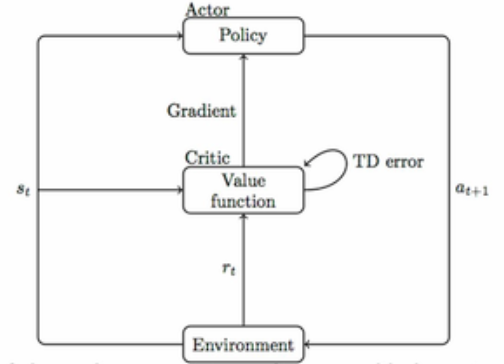
\includegraphics[width=0.5\textwidth]{images/aca.png}
  \caption{Actor-critic framework}
\end{figure}
\begin{itemize}
    \item Paramaters of the policy move to make a more likely action that has positive ``advantage'' - how much better is an action compared to a weighted average over all actions. $$A(s,a) = r(s,a) + \gamma \mathbb{E}[v(s') | s,a] - v(s)$$
    \item \cite{ODoherty04}: fMRI evidence that dorsolateral striatum (?) implements an actor ventral straitum (?) a critic.
\end{itemize}

Main of hierarchical reinforcement learning: A dinner cooking robot:
\begin{itemize}
    \item High-level steps: Choose a recipe, make a grocery list, \ldots
    \item Medium-level steps: get a pot, put ingredients in the pot stir until smooth, \ldots
    \item Low-level steps: precise movements of appendages
    \item All have to be seamlessly integrated\ldots
\end{itemize}
Many time-scales, many spatial scales, sensory (multi-modal) scales, etc, \ldots. Subtle changes in environment (e.g. cats) necessitate reactions in real-time. Abstract concepts, cause and effect. \\

\textbf{Options Framework}\cite{Sutton98}: generalizing the notion of actions - we would like something like a controller in continuous time
\begin{itemize}
    \item An option is defined by a tuple $\langle I_\omega(s), \pi_\omega(a|s), \beta_\omega(s) \rangle$
    \item initiation function (precondition)
    \item internal policy (behavior)
    \item termination function (post-condition)
\end{itemize}
E.g. robot navigation: if no obstacle in front (precondition) go forward (behavior) until something is too close (termination). Unlike classical MDPs/SMDPS, the options framework over an MDP considers multiple levels of abstractions [what about hierarchical contextual bandits framework?] \\

\cite{Botvinick08} propose some neural correlates of options \\

How can we think of options? ``little behavioral programs'' that come with predictive knowledge that can be learned via TD-error updates. \\

Intermediate result: option models speed up planning \\

Generalized actions, now generalize value functions - generalized rewards (many reward functions) \& continuation functions (depends on states). Given a cumulant (state-action context) function $c$, state-dependent continuation function $\gamma$, and policy $\pi$, a generalized value function is defined to be 
$$v_{\pi, \gamma, c} = \mathbb{E}[\sum_{k=t}^\infty C_{k+1}\prod_{i=t+1}^k \gamma(S_i)|S_t = s, A_{t:\infty}\sim \pi]$$
See Horde Architecture \cite{Sutton11} \\

Example: Successor Representations - discounted occupancy of a state (\cite{Dayan93, Barreto16}). Represents each state as a distribution over future trajectories from that state - vector-valued GVFs where features are cumulants. 
\begin{itemize}
\item spatial property \cite{Barreto16}: $v_{w^Tc,\gamma,\pi}(s) = w^Tv_{c,\gamma,\pi}(s)$
\item \cite{Gardner2018}: maybe dopamine yields a vector-valued signal for updating successor representations (?)
\end{itemize}

Frontier: Option Discovery - Options can be designed (e.g. pre-programmed controllers in robotics), subgoals or secondary reward structures can be provided \cite{Sutton98}, intrinsic motivation. \\

Bottleneck states: \cite{Solway2014} discover bottleneck states in navigation graph \& neural correlates, \& \textbf{random subgoals} require time \& data \cite{mann15} [what about self-supervised learning \& transfer-learning?], option-critic architecture \cite{BaconHP16} - results match or exceed Q-networks on atari. \\

\textbf{Conclusions}
\begin{itemize}
    \item Reinforcement learning has been a bridge between CS, NS, Cog-Sci
    \item Hierarchical reinforcement learning is a natural approach for solving large problems efficiently
    \item Deliberation cost and intrinsic rewards help learning
    \item learning jointly across temporal and state representations is beneficial \cite{Franklin2018}
    \item efficient option discovery is future work
    \item how can we model continual learning effectively?
\end{itemize}

\textbf{Questions} \\

Q. Automatic selection of options? \\

A. Option critic takes as a parameter the number of options and uses any actor-critic algorithm for learning the options. The main problem is reward optimization $\rightarrow$ options not necessary since policy will be sufficient, so options ``dissolve''. Need to give a little more knowledge/penalization/regularization to penalize switching/termination to encourage options to ``stay long''. Can also provide curiosity/intrinsic motivation/subgoals. No formal methods for deciding subgoals. \\

Q. Is it possible to combine the options framework with deep learning? \\

A. Option-critic architecture is a deep RL architecture. Using RL to drive the learning in the deep network exactly in the way you learn a value function via backprop.

%%%%%%%%%%%%%%%%%%%%%%%%%%%%%%%%%%

\subsubsection{9:00 - 9:30 Invited Talk: Deep learning without weight transport by \textit{Dr. Tim Lillicrap}}

Q. What are the fundamental principles of computational neuroscience? \\

A. Network architectures, loss functions, learning rules, environment/data (to a lesser extent)? \\

Q. Why these things? \\

A. Don't know how to understand neural architectures that recognize objects, but can understand how to build them (interested in principles). We know of and want learning rules that are powerful enough to solve hard problems (i.e. we know that the brain solves hard problems) and \textbf{respect biological constraints}. \\

One problem Brains have: credit assignment (given sensory information to be transformed into a judgement, in order to make good adjustments to synaptic connections, need to know what the associated judgments are). Solution used in NNs is backprop. \\

Credit assignment via backprop works well in practice, but doesn't respect biological constraints. 
$$ 
\delta W_0 \propto e\cdot W_1^T \cdot \sigma'(u) \cdot x
$$
Q. Why? \\

A. (1) Error term (2) \textbf{transpose of downstream weights} (``downstream'' knowledge \cite{Grossberg87}, weight transport problem) (3) derivative of activation function (normal neurons have spiking) (4) Separate forward and backward passes (synchronization) \\

More likely algorithms are weight perturbation \& activity perturbation - correlating noise in the synapse with changes in the error (but really slow in practice) \\

Q. Do/can existing biologically-motivated learning algorithms scale up to solve hard credit assignment problems? \\

Constraints on learning rules:
\begin{itemize}
    \item \textcolor{green}{No weight transport (e.g. with weight transposes)}
    \item \textcolor{yellow}{No weight tying (e.g. with convolutional kernels)}
    \item \textcolor{red}{Feedback of signed errors?}
    \item \textcolor{red}{Use continuous (rather than spiking) signals}
    \item \textcolor{red}{Violate Dale's law}
    \item \textcolor{red}{Local activation derivatives}
    \item \textcolor{red}{Separate forward/backward passes}
    \item \textcolor{red}{Your personal complaint here...}
\end{itemize}

A. Short story: \textbf{NO} \cite{Bartunov18} \\

Two approaches that learn the backward pathway \cite{Akrout19}: 
\begin{itemize}
    \item Weight mirrors: Directly learn transposes in a mirroring phase
    \item Kollen-Pollack (1994): Update both forward and backward weights using the same rule, and rely on weight decay
\end{itemize}

Weight Mirroring: described by two modes. \\

``Engaged mode'' (like backprop):
\begin{itemize}
    \item $\delta_l = \phi'(y_l)B_{l+1}\delta_{l+1}$
    \item $\Delta W_{l+1} = -\eta_W \delta_{l+1}y_l^T$
\end{itemize}
``Mirror mode'' (like hebbian updates):
\begin{itemize}
    \item $y_l \sim N(0,I)$
    \item $\Delta B_{l+1} = \eta_B \delta_l \delta_{l+1}^T$
\end{itemize}

Why weight mirroring works [linear case, for nonlinear case see paper]
\begin{itemize}
\item $\Delta B = \eta xy^T = -\eta \frac{\delta f}{\delta B}$
\item $x \sim N(0,I), y = Wx$
\item $\mathbb{E}[xy^T] = \mathbb{E}[xx^TW^T] = \mathbb{E}[xx^T]W^T = \sigma^2 W^T$
\item Decay $W$s to prevent divergence
\end{itemize}

Kolen-Pollack update (no modes): 
\begin{itemize}
    \item $\Delta B_{l+1} = -\eta y_l \delta_{l+1}^T$
    \item $\Delta W_{l+1} = -\eta_W \delta_{l+1} y_l^T - \lambda W_{l+1}$
    \item $\Delta B_{l+1} = -\delta_W y_l \delta_{l+1}^T - \lambda B_{l+1}$
    \item Note both $W$ and $B$ are decayed
\end{itemize}

Nice results for both methods on a deep network! Perform virtually as well as well-tuned backprop (drops correspond to learning rate schedule). \\

\textbf{Conclusions} 
\begin{itemize}
    \item Constraints from both sides are being met
    \item New machine learning algorithms that obey known constraints of biology and still perform well on hard tasks 
    \item Neuroscience experiments aimed at explicitly identifying the role of feedback in synaptic plasticity.
    \item Need to hold ourselves accountable when developing new algorithms
    \item Backprop-like mechanisms appear to be crucial for learning complex functions with deep networks
    \item To make effective weight updates, the structure of the downstream function should be communicated upstream
\end{itemize}

Addendum: How should we infer principles in the brain?
\begin{itemize}
    \item How should be make inferences about the underlying \textit{architecture}, \textit{loss}, and \textit{learning rules} in the brain?
    \item What would a scalable approach to inference look like?
    \item What neurological data should we collect to feed these inference processes?
    \item Can we learn to do this in-silico? [e.g. recovery of learning rules from simulated data]
\end{itemize}

\textbf{Questions} \\

Q. What's known about the accuracy to make the Pollack algorithm work? \\

A. Nothing is known about the accuracy. Global correlative signal may not be sufficient to learn to solve hard problems. Backprop may be good enough. 

Q. What dimensionality of error signal do you need to be able to send backwards to learn hard problems? \\

A. The answer may be unknown. E.g. what can you get away with to learn to solve imagenet?  \\

Q. What do you think about recent methods relaxing activations - noisy/auxiliary variable approaches. Address the issue of noisy activations (method of auxiliary coordinates, etc.) \\

A. Have their origins in the mid-late 80s - see O'Reily, 96 who looked at these relaxations seriously. One issue encountered is that these methods are slow, and the relaxations have to be ``long'' to perform on hard tasks. Hard to scale on hard problems/deep networks \\

Q. Backprop \& modeling the brain in a supervised setting. Want to prefer unsupervised methods. \\

A. whether you do VAE/GAN/etc. - all are using backprop to do credit assignment. Not using ``labeled errors', but still using backprop. Kind of stuck with backprop for credit assignment in deep networks. The question is how to do local credit assignment in a large network as you do unsupervised learning? \\

%%%%%%%%%%%%%%%%%%%%%%%%%%%%%%%%%%

\subsubsection{9:30 - 9:45 Contributed Talk: Eligibility traces provide a data-inspired alternative to backpropagation through time. \textbf{Guillaume Bellec}, Franz Scherr, Elias Hajek, Darjan Salaj, Anand Subramoney, Robert Legenstein, \textit{Wolfgang Maass}}

``Agree with Tim Lillicrap - NNs are a good tool to benchmark learning algorithms on machine learning problems because I realize they are not all functional and there is a lot hidden in that a lot of algorithms are functional and a lot are not.'' In this talk, Recurrent Neural Networks are the focus and we provide an alternative to Backpropagation through time. \\
\begin{figure}
  \centering
      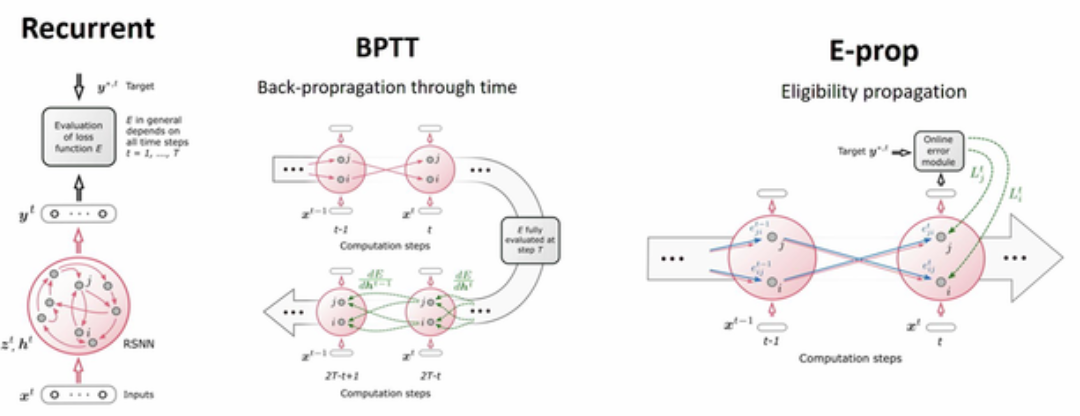
\includegraphics[width=0.5\textwidth]{images/eprop.png}
  \caption{}
\end{figure}

Biological motivation for e-prop (eligibility propagation \& Hebbian Learning) review from \cite{Gerstner18} the protocol to measure synaptic plasticity in the brain poke electrodes in pre and post-synaptic neurons \& look at... \\
\begin{figure}
  \centering
      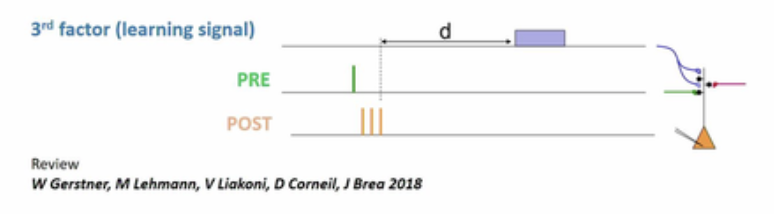
\includegraphics[width=0.5\textwidth]{images/3fl.png}
  \caption{}
\end{figure}

\textbf{Definition} Eligibility Traces: An abundance of trace events in the recent past in the internal states of neurons and synapses of the brain, often referred to in models as \textbf{eligibility traces}. \\

A lot of empirical support for significant delay between pre and post-pairing. \\

BPTT: forward propagation over entire sequence, backpropagate errors through unrolled recurrent network. - not acceptable for Brain. \\

E-prop - Top-down learning signal ($L_j^t$) based on a new ``local'' factorization of the loss gradient. \\

Given any loss function $E$, compute the gradient as $\frac{dE}{dW_{ji}} = \sum_t L_j^te_{ji}^t$ where $L_j^T$ is the learning signal and $e^t_{ji}$ is the eligibility trace, 
$$\frac{dE}{dW_{ji}} = \sum_t \frac{dE}{dz_j^t}\cdot[\frac{dz_j^t}{dW_{ji}}]_{local}$$
where $z_j^t$ is the (spiking - \textbf{new}) neuron output. \\

\textit{Proof sketch}:

given hidden state $h_j^t$ (voltage or memory cell dynamics) and observable state $z_j^t$ (spike of LSTM output), 
\begin{itemize}
    \item Separate (isolate) the hidden neural dynamics $\frac{\delh_j^t}{\del h_j^{t-1}}$ from the observable ones & push into eligibility trace
    \item Interchange two sums, to propagate hidden dynamics forward and the rest backward.
\end{itemize}

[see the paper for full proof, complexity analysis, & comparisons] \\

In practice, require online approximation of the learning signal since future is masked (unknown), but eligibility traces can still do hard credit assignment with delayed feedback. \\

Next slides on derivation of Reward-based e-prop from TD-Errors (RL-based, not fully supervised) experiments on Atari games [similar performance to A3C algorithms]. \\

\textbf{Conclusions} 
\begin{itemize}
    \item A new factorization of the error gradient in RNNs avoids BPTT and becomes compatible with the three-factor learning rule framework
    \item E-prop approaches the performance of BPTT in machine learning benchmarks
    \item Experimental prediction: comparing notion of eligibility trace to standard RL-version of ET are different due to notion of temporal neural dynamics (?)
\end{itemize}

\textbf{Questions} \\ 

%%%%%%%%%%%%%%%%%%%%%%%%%%%%%%%%%%

\subsubsection{10:30 - 11:00 Invited Talk: Computing and learning in the presence of neural noise by \textit{Dr. Cristina Savin}}

Interface between machine learning and neuroscience: building parallels between artificial and biological circuits - often the focus is on similarity \& points of contact. This talk focuses on a fundamental difference: the precense of intrinsic noise. Trained neural networks correspond to deterministic functions. NOT the case for biological neurons across brain regions, which may react differently to repeated identical stimuli ``neural variability''. What does this computation mean? \\

Inescapable ``bug'' of biological wetware: the main computational challenge that the brain faces is overcoming its own internal noise via active reconfiguration. \\

Feature: Intrinsic stochastic can be recruited for useful computational goals, e.g. representing uncertainty.  \\

This talk will introduce stochasticity for learning. 
\begin{figure}
  \centering
      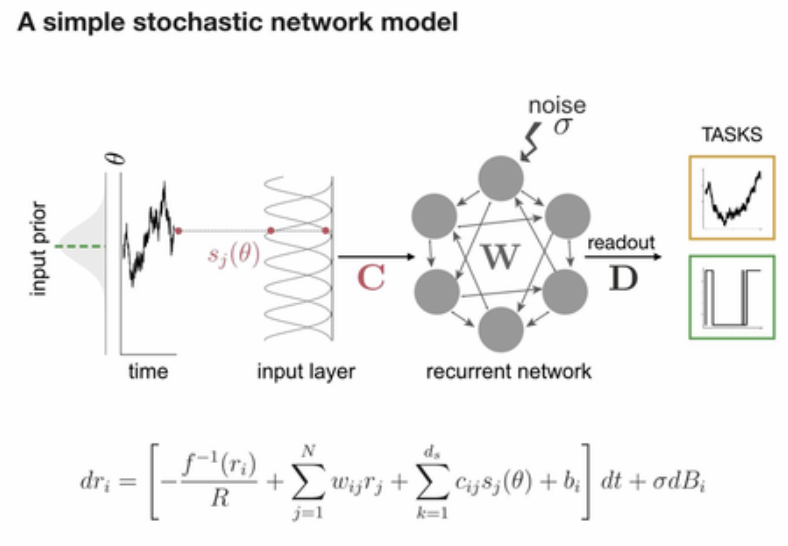
\includegraphics[width=0.5\textwidth]{images/stochnn.png}
  \caption{Stochastic NN \& two tasks: autoencoder \& binary classification}
\end{figure}

Adding brownian noise too each neuron independently in the neural network.

Goal: optimize \textcolor{blue}{task-specific} objective under \textcolor{green}{biological constraints} (regularization):
$$
O(D,W) = \int \textcolor{blue}{\alpha(Dr, s)}p(r|s(\theta),W)p(\theta)drd\theta - \textcolor{green}{\lambda ||W||_2})
$$
Network responses: $p(r|s(\theta),W) - \frac{1}{Z}e^{-\frac{E(r;s,W)}{\sigma^2}}$ and can write $E$ also in closed form (see paper). \\

Deriving optimal learning (gradient ascent) \cite{Williams1992, Fiete2006, Fiete2007, Scellier16, Miconi2017}:
$$
\delta w_{ij} \propto \textcolor{blue}{\alpha(Dr,s)}\textcolor{green}{(r_ir_j - \langle r_ir_j \rangle_{p(r|s)})} - \textcolor{red}{\lambda w_{ij}}
$$
\begin{center}
\textcolor{blue}{reward} - \textcolor{green}{Hebb} - \textcolor{red}{resource constraint}
\end{center}

This is relevant to adding noise independently to neurons (?) \\

\textbf{Conclusions}
\begin{itemize}
    \item Learning reshapes energy landscape in interesting ways to compensate for noise (by increasing firing rates preferentially for more likely stimuli
    \item some noise is needed for learning but bad for encoding
    \item More noise in the encoder $\rightarrow$ slower learning, poorer convergence due to variance of the gradients 
    \item Intrinsic stochasticity needed for task-dependent learning
    \item Active compensation of negative effects of noise
    \item (limitation) Instantaneous feedback $\rightarrow$ temporal credit assignment
    \item (limitation) Symmetric connectivity $\rightarrow$ asymmetric
    \item (limitation) Variance of gradients $\rightarrow$ more biological detail
\end{itemize}

\textbf{Questions} \\

Q. More probable stimuli require more neurons how is it relevant to shannon code theory (more probable strings $\rightarrow$ smaller code). Is there a loss in efficiency? \\ 

A. Depends on the spectrum of constraints \& magnitude of the noise. Recurrent noise. \\

Q. Found noise aligns significantly in the coding manifold. Can you disambiguate - what is the code and what is the signal? \\

A. Equating the two - the output of the network is the only thing that matters.

%%%%%%%%%%%%%%%%%%%%%%%%%%%%%%%%%%

\subsubsection{11:00 - 11:30 Invited Talk: Universality and individuality in neural dynamics across large populations of recurrent networks by \textit{Dr. David Sussillo}}

Treatment: neural networks as artifical model organisms. Can train neural networks to accomplish tasks analogous to those studied in animals, full spec. of paramters (as opposed to brains), utilize optimization, reverse engineering, ability to conduct huge experiments. \\

\cite{Churchland2012, Sussillo2015} a debate in systems neuroscience about whether or not firing rates in motor cortex encode kinematic parameters (target, location, velocity, etc.) or if there is an underlying dynamical system [LFADS].  \\

Experiments provide a supporting sufficiency argument that driving muscles produces activations that look like motor cortex (many examples of using nns to understand how the brain functions - first is \cite{Zipser1988}) \\

The big assumption: Why do biological and artificial representations look similar in many cases?
\begin{itemize}
    \item similar components and learning rules?
    \item universality?
    \item if universalty in what sense?
    \item a unique solution for all networks, a set of solutions classes or is each network unique?
\end{itemize}

Universality: e.g. Feigenbaum's delta\footnote{\url{https://en.wikipedia.org/wiki/Feigenbaum_constants}}

Want to study a lot of RNNs \& learned architectures. Are any of these architectures better at reproducing neural dynamics compared to others? Yes! Studied 1000s of networks and systematically analyzed then by studying representational geometry (cca), fixed point topology, and linearized dynamics around fixed points. \\

Many experiments on several simple tasks: 3-bit memory, oscillatory tasks speak to pattern generators, integration task speaks to decision making in the brain. \\

Identified structure via CCA among different network types.
\begin{figure}
  \centering
      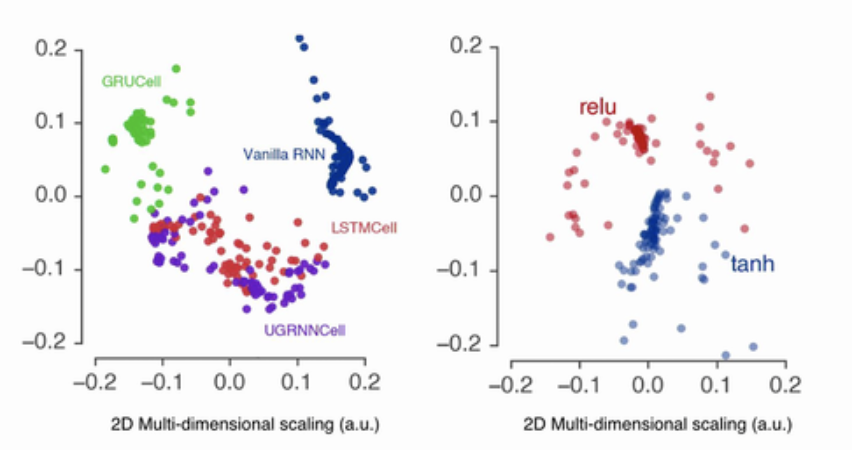
\includegraphics[width=0.5\textwidth]{images/nnclust.png}
  \caption{Clusters of different RNN-type architectures trained on simple tasks}
\end{figure}

\textbf{Definition} Fixed point: 
\begin{itemize}
    \item $h_t = F(h_{t-1},x)$
    \item $h^* = F(h^*, x^* = 0)$
\end{itemize}

Can study linearized dynamics (recovered numerically) around fixed points. \\

\textbf{Conclusions}
\begin{itemize}
\item Representational geometry differs between models.- thus geometry may be useful in piking models closer to biological circuits
\item The underlying fixed point topology may still be the same in the RNN (e.g. all models had line attractors in the integration task)
\item Linearized dynamics appear very similar although minor differences
\item These two may indicate universal solutions, and provide useful invariants across all networks
\item These issues are foundational if we are going to continue using deep learning to understand neurobiological data (and same holds true more generally for other types of data)
\end{itemize}

\textbf{Questions} \\

Q. Be careful with what is called universality  \& results may come from the tasks. \\

A. I disagree - the tasks do define the structures, but there do seem to be structures that are not hand designed over all the networks. \\

Q. Did you consider looking at the dynamics of systems that did not converge/were not trained/partially trained. \\

A. No, but that is a great line of future research. 

%%%%%%%%%%%%%%%%%%%%%%%%%%%%%%%%%%

\subsubsection{11:30 -11:45 Contributed talk: How well do deep neural networks trained on object recognition characterize the mouse visual system? \textit{Santiago A. Cadena}, Fabian H. Sinz, Taliah Muhammad, Emmanouil Froudarakis, Erick Cobos, Edgar Y. Walker, Jake Reimer, Matthias Bethge, Andreas Tolias, Alexander S. Ecker}

\textbf{Main question}: What is the function of the multiple visual areas of the mouse brain? and is there a clear object processing pathway in the mouse visual cortex? \\

We know that neighboring points in visual space map to neighboring points in cortical space \cite{Wang2007}. \\

Record $\sim$5000 neurons per area in visual area in response to $\sim$5000 images from iamgenet. Interested in mapping from input image + other variables to neural responses. The other variables include running speed, pupil dilation and pupil directions. The mapping function is chosen to be a convolutions neural network (VGG-16). Recover the hypercolumns. \\

C1. What is the right resolution of input images? \\

C2. Performance is sadly flat w.r.t hierarchical correspondence between VGG layers and neuronal activity. \\

C3. Is the model describing responses at all? - Captures between 70 and 80 percent of variation \& exceed the performance of classical model. \\

C5. Taking the exact same architecture with rith random weights, performance is pretty similar. - Is the goal with what you are training the network driving performance for predicting neural activity? - The number of layers is critical to match neural activity. \\

\textbf{Conclusions}
\begin{itemize}
    \item Optimizing input resolution is critical for layer-to-area correspondence
    \item Models with random features can be baselines for goal-driven modeling
    \item Static object recognition does not appear to be the right goal to characterize the functional organization in mouse cortex
    \item We need visually guided tasks that are more ethnologically relevant. 
\end{itemize}

\textbf{Questions} \\

Q. Do you think that the high dimensionality of the hidden representations of VGG could drive the performance of the random network - did you try narrower networks? \\

A. Yes absolutely. \\

Q. What about single neuron-to-neuron comparisons? \\

A. Not sure \\

Q. Why not feed the same resolution - why can you optimize the resolution? \\

A. Not sure what the pixels of degree resolution for visual field (?)

%%%%%%%%%%%%%%%%%%%%%%%%%%%%%%%%%%

\subsubsection{11:45 - 12:00 Contributed talk:  Functional Annotation of Human Cognitive States using Graph Convolution Networks \textit{Yu Zhang}, Pierre Bellec}

\textbf{Main question}: What is an efficient way of doing brain decoding and understand brain cognition? \\

Want to try using deep learning - GCNNS - to recover universal representation space for multiple modalities - use Human Connectome Project data \cite{Hughes2016}. \\

Project fMRI data onto a brain graph and apply GCNNs. Use Guided Backpropagation to generate saliency maps. - Able to identify regions involved in language processing, visual processing, motor tasks, etc. Compare different models, different ways of composing the graph. \\

\textbf{Questions} \\ 

Q. What's the motivation for using GCNs as opposed to classical image analysis techniques? \\

A. Memory constraints \\

\textbf{Questions} \\

%%%%%%%%%%%%%%%%%%%%%%%%%%%%%%%%%%

\subsubsection{14:00-14:30 Invited Talk: Simultaneous rigidity and flexibility through modularity in cognitive maps for navigation by \textit{Dr. Ila Fiete}}

\textbf{Outline:} \\
Invariance/rigidity: the brain contains intrinsically low-dimensional representations that are invariant and rigid. \\

Flexibility: principles by which invariant/rigid modules can provide high efficiency and flexibility. \\

General non-Euclidean semantic inference using grid and place cells. \\

Plug for Kernel RNN learning (KeRNL): simple, biologically plausible alternative to BPTT \cite{roth2018kernel} \\

Apply topological data analysis to show a $\sim$2000 neuron circuit \cite{Chaudhuri2019} lie on a 1D ring during unconstrained activity \& during REM sleep via topological data analysis \& co-embedding. \\

%%%%%%%%%%%%%%%%%%%%%%%%%%%%%%%%%%

\subsubsection{14:30 - 15:00 Invited Talk: Theories for the emergence of internal representations in neural networks: from perception to navigation by \textit{Dr. Surya Ganguli}}

Lots of success with training neural networks to solve tasks and comparing internal representations to those in neural networks. \\

Replacing something we don't understand with something else we don't understand? \\

Trained a CNN to mimic salamander retina responses to natural scenes with good results - able to model retinal activity across salamanders. \\

Try to go from deep networks to simple and interpretable subcircuits that are essential for generating reponses from stimuli via model reduction. Able to map these subcircuits to neuronal circuits. \\

\textbf{Conclusions}
\begin{itemize}
\item Interpretable deep learning for the brain through model reduction
\item Explaining the structure of the retina through auto-encoders
\end{itemize}

\textbf{Questions} \\

Q. Biological constraints \\

A. We also used weight decay, etc.

%%%%%%%%%%%%%%%%%%%%%%%%%%%%%%%%%%

\subsubsection{15:00-15:15 Contributed talk: Adversarial Training of Neural Encoding Models on Population Spike Trains \textit{Poornima Ramesh}, Mohamad Atayi, Jakob H Macke}

Neural activity is driven by both stimulus (signal) and latent variables (noise). \\

Q. How to build a generative model to match real data? \\

A. Use GANs. \\

If we have such such a model we can use it to explore model complexity and recover synthetic data for stimulation and perturbation experiments. \\

Q. How to backprop through spike trains? \\

A. Use gradient estimators - e.g. concrete relaxation (biased generator output) \cite{Maddison16}, REINFORCE (good result) \cite{Williams1992}, and REBAR: REINFORCE + concrete relaxation as a control variate (comparable to REINFORCE). \\

\textbf{Issue}: results given for training data, couldn't get GAN to generalize on test data - did generalize on heteroscedastic synthetic data. \\

\textbf{Summary} \\
Attempt to capture both signal and noise in neural populations using GANs trained via REINFORCE. Future work extends the framework to recurrent or dynamical spiking models and transfer learning and comparison with other deep latent models.

\textbf{Questions} \\

Q. What were the problems generalizing to the test data? \\

A. Managed to get noise correlations, but not able to capture PSDH (time-varying firing rate) - possibly low data SNR. \\

Q. Why not use VAEs which naturally support discrete outputs? \\

A. Future work.

%%%%%%%%%%%%%%%%%%%%%%%%%%%%%%%%%%

\subsubsection{15:15-15:30 Contributed talk: Learning to Learn with Feedback and Local Plasticity \textit{Jack Lindsey}}

Q. Are deep neural networks a reasonable model of brain function - in particular learning?
\begin{itemize}
    \item Deep learning can solve hard tasks
    \item Trained deep networks with appropriate constraints often exhibit brain-like representations
\end{itemize}
A. Not quite - see the earlier talk by Tim Lillicrap. \\

Propose a meta-learning approach. \\

\textbf{Core idea}: To make a biologically plausible learning work 
\begin{enumerate}
    \item Define the space of biologically plausible learners of interests
    \item Meta-learn over that space
\end{enumerate}
The hope is that by introducing feedback matrices, we enable deep credit assignment which enables doing more than just feature reuse (and maybe tells us something about biological credit assignment). \\

Tried this approach on two ``families'' of tasks: multiple sinosoidal regression and one-shot classification tasks with hebbian inner updates and varying number of ``plastic'' layers. \\

\textbf{Questions} \\ 

Q. You meta learn both the initialization weights and feedback weights? \\

A. I guess if you started mixing and matching you might have trouble, but not learning feedback weights doesn't work as well, but it also doesn't fail completely. \\

Q. Have you incorporated synaptic pruning? \\

A. No direct mechanism in the current implementation - maybe implicit, but interesting future work to include pruning, recurrence, neuromodulation, etc. \\

%%%%%%%%%%%%%%%%%%%%%%%%%%%%%%%%%%

\subsubsection{16:45-17:15 Invited Talk: Sensory prediction error signals in the neocortex by \textit{Dr. Blake Richards}}

Presentation on data and how to incorporate machine learning into neuroscience - cost functions, learning rules involved in neuronal circuits. \\

Question: Does the neocortex try to predict incoming stimuli using top-down connections (i.e. a hierarchical generative model) and does it use prediction errors for credit assignment? \cite{Lotter16}. \\

Partial Answer: To answer this question experimentally we can't only look for signatures of prediction errors, we need to consider the specific architecture of the neocortical microcircuit \cite{Harris13}. \\

A lot of evidence suggests that our brains are sensitive to unobserved stimuli (L2/3) - e.g. \cite{Zmarz16, Homann17} reported that violations of expected visual flow induce strong responses in L2/3 neurons (2-photon calcium imaging) [Mice in a virtual reality environment!]. \\

Three unresolved questions \cite{Harris13}:
\begin{itemize}
    \item What is happening in the apical dendrites that are receiving the top-down inputs
    \item What is happening in the other cells in the microcircuit that can project up the hierarchy?
    \item What happens over the course of time, and over multiple sessions of exposure to unexpected stimuli?
\end{itemize}

\textit{Proposal for data accepted by the Allen Institute for Brain Science OpenScope program.}\footnote{link}
 \begin{itemize}
     \item Randomly re-oriented Gabor sequences
     \item Hallway visual flow perturbations
     \begin{figure}
  \centering
      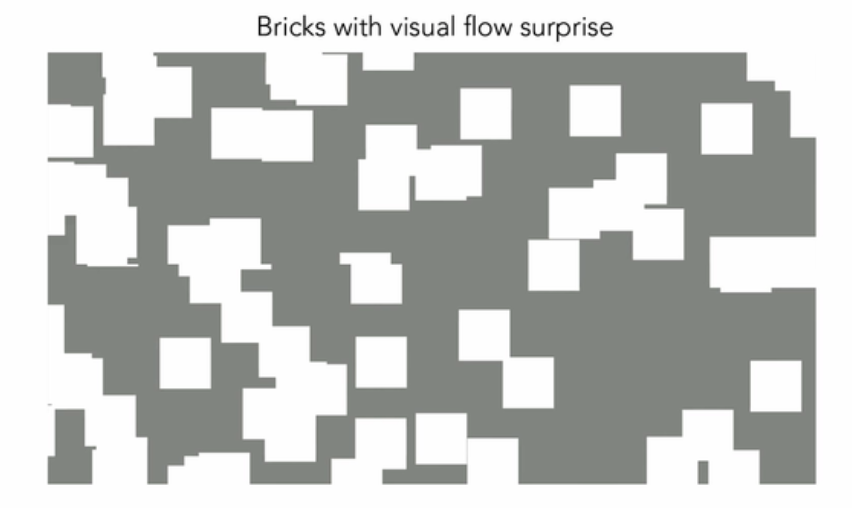
\includegraphics[width=0.5\textwidth]{images/hallway.png}
  \caption{Hallway visual flow perturbation, couldn't get a pic of the Gabor orientation task.}
\end{figure}
 \end{itemize}
 
Recovery of perturbations - ``stimulus direction'' is possible by linearly decoding latent neuronal activity (better than chance for ~2-dozen data points), responses not driven by running increases or pupil dilations, although both lead to higher df/F. \\

Interestingly, increase in neuronal activity for subsequent trials for Gabor task. \\

\textbf{Conclusions} \\

The open-loop data supports the idea that there are prediction error signals driven by top-down info, with different parts of the circuit engaging in different computations. \\

The cumulative data in the field points strongly towards an unsupervised predictive hierarchical model in the neocortex. \\

The next steps are to further understand the different parts of the circuit and determine how it is learning. \\

\textbf{Questions} \\

Q. Why no L4 neurons to understand top-down processing? \\

Richards: Reasonable next step. We didn't do it. Would like to see experiments reproduced in all cell-types. \\

Q. What is the somatic responses look like when the error responses are happening? \\

Richards: Found a lot of variability in synaptic responses, but L5 pyramidal neurons showed fairly ``clear'' response in burst session that died over time - didn't mention it due to variability. \\

Q. A related study from Princeton demonstrated specific responses (specific neuronal activity) did you find this? \\

Richards: Generally, different ROIs respond to different orientations, which is why we can decode. For the hallway, was some specificity, but no clear split between ``error neurons' and ``non-error neurons'' \\

%%%%%%%%%%%%%%%%%%%%%%%%%%%%%%%%%%

\subsubsection{17:15 -18:00 Panel Discussion: A new hope for neuroscience}

Pannelists: Yoshua Bengio, Blake Richards, Timothy Lillicrap,  Ila Fiete, David Sussillo, Cristina Savin, Konrad Kording, Surya Ganguli \\

Goal: explore future directions surrounding the intersection of AI and neuroscience \\

Q. True or false: to truly understand the brian, one needs to study artifical intelligence.  \\

A. \textbf{T: } BR, IF, YB, TL $\mathbf{\sim}$\textbf{:} CS, SG \textbf{F: }DS \\

SG: It's important to study the problems that are being tackled in AI and to understand the space of solutions - not necessarily overfit to solutions in AI. AI techniques are tractable and can be used to solve hard problems, but need to explore other possibilities. \\

BR: Agree, broad question: are there general principles of intelligence (I think there are) one way is to engineer systems that behave in an intelligent manner. AI $\rightarrow$ engineer intelligent systems, Neuro $\rightarrow$ understand biological mechanisms that underpin intelligence. Seems like both are needed to get at general principles that apply to both. \\

CS: What do people mean about understanding brains? Understanding intelligence? E.g. mechanistic models \&  clinical models may not need AI to undestand the brain. \\

DS: Pedantic - probably don't \textbf{need} to study AI. It's also possible that AI could mislead us. \\

YB: Current ways of thinking of researchers in machine learning focus on statistical questions - the learning problem and on what sorts of constraints this imposes on what works and what doesn't work - why would evolution put particular structures in the brain brings a useful and important light to understanding the brain - whether or necessary or not is not as important. For ML you have to think this way, but maybe in the future Comp-neuro may not need to talk to ML people. \\

Q. Many talks can be categorized into two categories: (1) how does computation happen (2) get after learning rules that shape computation. What do you think about the prospect of studying computation as they can be observed in the brain in trained neural networks as opposed to learning rules. \\

YB: Super important - what the whole field of machine learning is telling us is that the particular kind of computations that work or don't work do the job in the context of learning - imposing some kind of prior on the solutions that the brain may need to find in natural environments. Cannot disassociate the computation - which has to do with the final product (what you have learned) - from why you end up with that particular form of computation. From a computer science perspective, you can implement the same function many ways. Families of functions/architectures which make learning easier, faster. For biology and evolution this is a huge advantage w.r.t a need for fast learning. \\

IF: We definitely don't fully understand learning rules - in particularly unsupervised. But a lot of structure and modularity in the brain & inductive biases. \\

YB: Disagree. Architectures matter because of the learning. Learning is not just the learning rule. Learning rules are just some computation on the circuit. The purpose of the whole thing is to facilitate the learning. You can't separate architecture for a particular function from synaptic mechanisms that do the learning. In ML, the purpose of all the pieces of the puzzle stand together to create systems that can learn efficiently. \\

TL: At least for complex problems (image classification, go), we have reasonable solutions in-silico by inscrutable networks. A focus on interpretation in neuroscience and AI would be great - and asking what understanding even looks like. \\

BR: Architectures are critical - understanding the architecture and the shapes is getting at the computation. Can't expect a little just-so story about every neuron in the brain. \\

SG: Thinks we are overfitting to our current understanding of AI systems. \\

BR: Disagree. If anything NNs will be worse than the brain - evolution has no motivation to produce ``scrutable stuff''. \\

SG: It does need to create robust stuff, but we hope robustness leads to scruitability. \\

TL: But what needs to lead to robust stuff? Representations, behaviors, \textbf{learning rules}, etc. \\

DS: Side point on learning rules \& computation: it's very important in NS to be constantly be making contact with data. Studying the computation is a far easier task from an experimental point of view. \\

YB: Modularity. A lot of DL on modularity - successful deep nets that have modular structure for which computation is not homogeneous - groups of neurons that talk to other neurons in a controlled way. E.g. Antonio Touralbla's group can identify layers that have semantic interpretation. Observing modularity in the brain may be possible, but recovering the computation may not make much sense. \\

BR: Agree w/ stay connected to the data, but data today suggests that single neurons are inscrutable. Majority of cells in circuit can't really interpret. Lots of data is just a hope. \\

TL: The question on my mind: what should we be doing with neurological data and what kinds of neurological data should we be aiming for? Data that describes architectures, learning rules, etc. We don't even know what understanding [brain ,nns] even looks like. \\

SG: Neuroscience has been weak on understanding the learning rules. \\

TL: The argument isn't to discover backprop in the brain. Need to let the data talk for itself. \\

Q. Thought experiment: with all the experimental processes in the world, what would be the one experiment to design? \\

TL: Can do exactly that with networks on a computer. \\

DS: If we can't make sense of these models on our computer, it may be hopeless for our brain - need to know what it means to understand something. \\

SG: Handicap ml - what if you can only measure the activities of neurons given the inputs, but you don't get the weights or connectivity of the network. \\

TL: My lab is working on this. \\

YB: About multiple modules that have different objectve functions - people in machine learning are studying this too (GANS, multi-agent learning within a system), studying how to go from a single object to a multi-agent-like setting. \\

Q. Appreciate biological theories to account for how the brain might work - also interested in neuromorphic computing on-chip. Rarely hear about this in the ML community. Do you believe in this approach? \\

YB: A lot of work, unfortunately these techniques ignore the ML perspective precisely. Jeff Hinton likes analogies: understand an build cars but you are aliens looking at the planet from far away, but you don't see the inside of the motors. You may try to build something that looks like a car, but turning the key $\rightarrow$ nothing happens. This is basically spiking NNs \& neuromorphic computing. Things are changing, though w/ efficient implementations, quantization, etc. \\

DS: Once we figure how to spiking NNs, neuromorphic computing may take off. \\

Q. Beyone neurmorphic chips, what are the key principles that we learn from neuroscience that might influence new principles in ml and visa-versa? \\

IF: Simple networks that exist in the brain and can be repurposed - reuse of multiple modules. \\

DS: Uncommon intuitions: we don't have a clue about how to handle memory in artificial systems. Biological influence may be reasonable. \\

YB: Agree. Piecewiselinear narrative came from (in my group) from something we thought was closed to neuroscience. Personally interested in what we can learn from neuroscience at the level of memory, attention, system-2 processing. Many things that can suggest techniques and explorations in ML. \\

BR: Critical. Architectures is a huge thing - architecture optimization is very difficult, and many of the most successful architectures (convnets) inspired biologically. \\

Done. Bye!! :)

\bibliography{nn}
\bibliographystyle{abbrv}

\end{document}
